\documentclass[11pt,a4paper]{article}
\usepackage[utf8]{inputenc}
\usepackage{amsmath}
\usepackage{amsfonts}
\usepackage{amssymb}
\usepackage{float}
\usepackage{graphicx}
\usepackage{todonotes}
\usepackage{algorithm}
\usepackage{algpseudocode}

\restylefloat{table}
\title{Project Report: Managing Transfer-Based Datacenter Connections}
\author{Daniel Naro, Maria Gabriela Valdes, Victoria Beleuta}
\begin{document}
\maketitle
\section{Introduction}
% to do: maybe add an example? make references and label sections

For our project we implemented the integer linear programming model described in the paper "Managing Transfer-Based Datacenter Connections" by Adrian Asensio and Luis Velasco. In order to accommodate spikes in cloud demand, while managing the energy consumption of datacenters, it is necessary for datacenter federations to be created. When building large infrastructures cloud operators, with the help of these federations, are capable of reducing capital expenditures by having a dinamic cloud service that uses under-utilized resources in remote datacenters. These dinamic cloud services the huge energy consumption in remote datacenters are minimized, because servers can be turned on and off as needed \todo{what?}. To implement these sort of elastic operations, cloud computing strongly depends on the interconnected datacenters through a network providing huge capacity and having the necessary resources available. The interdatacenter traffic results from workloads being encapsulated in virtual machines and moved on different data-centers. Because the amount of data that needs to be transferred is huge, data-centers are interconnected with a flexgrid optical network. Resource managers can set up and tear down connections of the necessary bitrate, for a specified time period needed to transfer the data. For each of these connections, the frequency slot, i.e. spectrum width, depends on the bandwidth requested and the used modulation format. Elastic connections were suggested due to the fact that not enough resources might be available at the request time, so the manager can dynamically modify the spectrum allocated (RSSA problem) \todo{isn't that the RSA problem?} to ongoing transferences and the requested connection to accommodate all traffic and complete it in the requested time. These elastic connections are possible through programmable bandwidth-variable transponders that can provide optical signals of different characteristics.\\

A different approach was proposed in \cite{1}, the author use carrier software defined network (SDN) controller on top of ABNO transforms requests from cloud resource managers into connection requests, which helps with a better understanding of network complexity. This paper further explores carrier SDN functionalities by using scheduling techniques in addition to elastic operations, which as a result increases network operator revenues by accepting more connection requests. The SDN controller computes the routing path and necessary spectrum for each transfer and decides the elastic operations that need to be done on ongoing transferences to fit the new transfer, while satisfying the completion time for all transfers.\\

The rest of our project report is structured as follows. We present the integer linear programming (ILP) model implemented in section 2. Section 3 and 4 defines two metaheuristic algorithms. The results of our project and a comparison of the results obtained are detailed in section 5. Finally, section 6 concludes the report.

\section{ILP Model}

In order to simplify the RSSA problem, we limited our project to only one new transfer being requested. We have a network topology represented by a graph $G(L,E)$ with a set of locations ($L$) and set of fiber connections ($E$). We are given a subset ($D$) of the data-centers' locations. We also know the characteristics of the connections, i.e. a set $S$ of available spectrum slices, and the capacity and number of flows of the optical transponders at each location. The set $R$ contains the ongoing transferences. For each transfer we know the origin ($o_{r}$), destination ($d_{r}$), the remaining amount of data ($v_{r}$) to be transferred, the requested completion time ($c_{r}$), the route ($r_{r}$) and slot currently allocated ($s^{0}_{r}$), the scheduled slot allocation ($s^{1}_{r}$) to be performed at time $t^{1}_{r}$, and the scheduled completion time ($t_{r}$). The details of the new transfer request are given in the tuple $\{o_{r}; d_{r}; v_{r}; c_{r}\}$. The output of our model is the route allocated ($r_{r}$), scheduled completion time ($t_{r}$), bitrate of the connection ($s^{0}_{r}$), the new spectrum allocation ($w^{0}_{r}$), scheduled reallocation ($w^{1}_{r}$, $t^{1}_{r}$), and completion time ($t_{r}$) for each transference that is rescheduled. Our objective is to minimize the number of connections to be rescheduled to make room for the incoming request.\\

% to do: do we need pseudo code for precomputing?
A rescheduling for any transference $r$ needs two spectrum allocations: $s^{0}_{r}$ from time $t_{0}$ to $t^{1}_{r}$ and $s^{1}_{r}$ from time $t^{1}_{r}$ to $t_{r}$, so that the combined area of the two rectangles allows conveying the remaining amount of data $v_{r}$ and $t_{r} \leq  c_{r}$. To decide dimensions, spectrum and time for the ongoing transferences are precomputed. To do this we have written a Java program which precomputes any feasible combination of rectangles $A_{0}$ and $A_{1}$. To obtain these rectangles, we consider discretized time. The sets of rectangles are generated for the ongoing transferences and the requested transfer.\\\\

\begin{algorithm}
\caption{Generation of rectangles}\label{rectangles_precomputation}
\begin{algorithmic}[1]
\Procedure{Rectangles\_precomputation}{$transfer, max\_slice$}
	\State $start\_time\_a0 \gets 0$
	\State $compliant\_rectangles\_pair$
	\For{$end\_time\_a0=1 \to transfer.dead\_line$}
		\For{$slice\_start\_a0=0 \to max\_slice$}
			\For{$slice\_end\_a0=slice\_star\_a0 \to max\_slice$}
				\State $tmp\_a0 \gets Rectangle(start\_time\_a0, end\_time\_a0,slice\_start_a0,slice\_end\_a0)$
				\For{$j=i \to transfer.dead_line$}
					\For{$slice\_start_a1=0 \to slice\_start_a0$}
						\For{$slice\_end_a1=slice\_end_a0 \to max_slice$}
							\State $tmp\_a1 \gets Rectangle(start\_time\_a1, end\_time\_a1,slice\_start_a1,slice\_end\_a1)$
							\If{$transfer.rectanglesCompliant(tmp\_a0, tmp\_a1)$}
								\State $compliant\_rectangles.add(tmp\_a0, tmp\_a1)$
							\EndIf
						\EndFor
					\EndFor		
				\EndFor
			\EndFor
		\EndFor		
	\EndFor
\EndProcedure
\end{algorithmic}
\end{algorithm}


In order to present the ILP model, we define the necessary parameters and variables:
\begin{table}[H]
\small
\begin{tabular}{c l}
$E$ & set of fiber links in the network, index $e$.\\
$S$ &  set of frequency slices, index $s$.\\
$T$ & set of time intervals, index $t$.\\
$R$ & set of ongoing transferences, index $r$.\\
$P$ & set of routes between origin and destination for the new request, index $p$.\\
$A$ & set of candidate areas for the requested trans- ference, index $a$.\\
$A^{0}_{r}$ & set of candidate areas for $r$ between $t_{0}$ and $t^{1}_{r}$ and a spectrum allocation.\\
$A^{1}_{r}$ & set of candidate areas for $r$ between $t_{1}$ and $t_{r}$ and a spectrum allocation.\\
$\omega_{ar}$ & 1 if transference r was assigned to area $a$, 0 otherwise.\\
$\delta_{as}$ & 1 if area a includes slice $s$, 0 otherwise.\\
$\gamma_{at}$ & 1 if area $a$ includes time interval $t$, 0 otherwise.\\ 
$\rho_{pe}$ & 1 if route $p$ uses link $e$, 0 otherwise.\\
$\rho_{re}$ & 1 if transference $r$ uses link $e$, 0 otherwise.\\
$\beta_{raa'}$ & 1 if pair of areas $a \in A_{0}$ and $a' \in A_{1}$ for transference $r$ is feasible.\\
\end{tabular}
\end{table}
Variables:
\begin{table}[H]
\small
\begin{tabular}{c l}
$x_{ap}$ & 1 if the new transference is assigned to area $a$ through route $p$.\\
$y_{r}$ & 1 if transference $r$ is rescheduled, 0 otherwise.\\
$x^{0}_{ar}$ & 1 if transfer $r$ is assigned to area $a \in A_{0}$.\\
$x^{1}_{ar}$ & 1 if transfer $r$ is assigned to area $a \in A_{1}$.\\
\end{tabular}
\end{table}
And the ILP model is as follows:\\
$minimize \sum_{r\in R} y_{r} $\\\\
subject to:\\
$\sum_{a \in A} \sum_{p \in P}$ $x_{ap} = 1$\\\\
$\sum_{a \in A_{0(r)}}$ $x^{0}_{ar}=1$    $\forall r \in R$\\\\
$\sum_{a \in A_{1(r)}}$ $x^{1}_{ar}=1$    $\forall r \in R$\\\\
$\sum_{a' \in A_{1(r)}}$ $\beta_{raa'}*x^{1}_{a'r} \geq x^{0}_{ar}$     $\forall r \in R,$ $a \in A_{0(r)}$\\\\
$x^{0}_{ar} - \omega_{ar} \leq y_{r}$     $\forall$ $r \in R,$ $a \in A_{0(r)}$\\\\
$\sum_{r \in R} \sum_{a \in A_{0(r)}}$ $\delta_{as} * \gamma_{at} * \rho_{re} * x^{0}_{ar} + \sum_{r \in R} \sum_{a \in A_{1(r)}} \delta_{as} * \gamma_{at} * \rho_{re} * x^{1}_{ar}$\\ 
$+ \sum_{a \in a} \sum_{p \in P} \delta_{as} * \gamma_{at} * \rho_{pe} * x_{ap} \leq 1$    $\forall$ $e \in E,$ $s \in S,$ $t \in {\{t^{0},...,T\}}$\\

The first constraint guarantees that the transfer request is served with route $p$ and rectangle $a$. Then we select the feasible rectangles for the ongoing transferences with the next three constraints. After words, with the sixth constraint we decide whether a transference needs to be reallocated or not and the last constraint guarantees that there are no links used by more than one constraint for each time interval. We have implemented and tested our ILP model with the ILOG CPLEX studio.

\section{Metaheuristic Algorithms}

To solve the spectrum allocation problem use the Greedy and GRASP algorithms. Initially we develop a programm to precompute all the available paths in the graph between source and destination nodes of the requested transfer using Breadth-first search. These paths are the candidates in our set $C$. Next, we have divided the search for a feasible solution in three main parts: Trivial Case, Half Hard Case and Hard Case, and we analyze in which category the addition of this new transfer falls into.\\

A trivial case, showed in Fig. 1, happens when adding a new transfer into the network does not require the rescheduling of any of the other scheduled ongoing transfers, because the required number of free slices is already available.

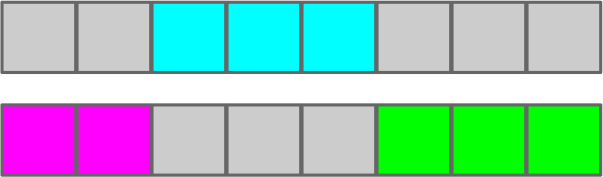
\includegraphics[scale=1]{trivialcase.jpg}

The half hard case, Fig. 2, implies evaluating the possibility of adding a new transfer into the network, but only some slices are currently available, but not enough. In this case it is necessary to check on each link, all of the ongoing transferences, and see if they can be rearranged to inclease the time it takes to end the transaction, while still maintaining the completion time constraint, consequently freeing up some slices for the requested transfer. We first check if “squeezing” the left transfer to the left we have enough space, if not we try “squeezing” the right transfer to the right and check again if we have freed all the slices needed by the new transfer. 

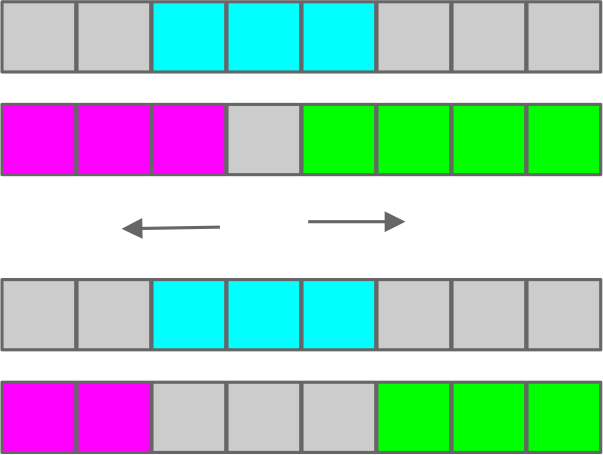
\includegraphics[scale=1]{halfhardcase.jpg}

When we do not have any free slices available in any link throughout the selected path, we have a hard case, Fig. 3. Adding a new transfer into the network requires all of the necessary slices to be freed. In this particular case, we have to perform the same “squeezing” procedure specified in the previous case, but first we have to check each intersection point between two ongoing transferences to select a starting point where we can insert the new transfer that needs to be scheduled. Once we have found an intersection which we can expand enough to make room for the requested transfer, we have to check on the other links if the expansion is also possible there. Once an insertion point, suitable on all links is found, we start performing the reschedulings.

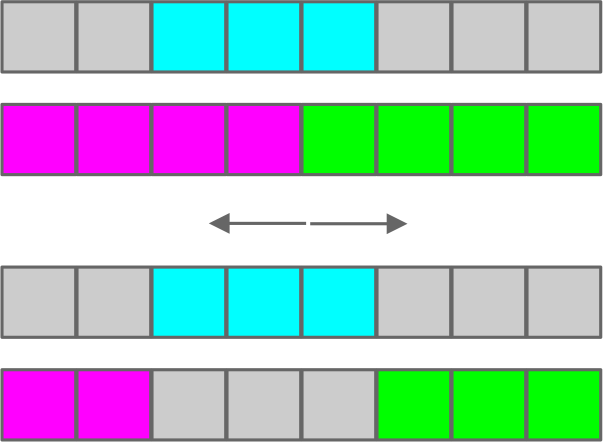
\includegraphics[scale=1]{hardcase.jpg}

 \subsection{Greedy}
For our first methaheuristic, we used the Greedy algorithm that iterates through all the precomputed paths, going through all the previously defined cases to find a feasible solution. If a solution is found for a given path, the loop termites and the rest of the paths are not checked.
 
 \subsection{GRASP}
Using the GRASP algorithm for the second metaheuristic, we define the greedy function and the RCL. We order the precomputed available paths by length or number of hop, and use an alpha parameter of 0.3 to select only the best subset of smallest found paths. Once the RCL is is found, we can start iterating. At each step, we select at random one of the paths within this array of paths.\\

The local search of our GRASP algorithm consists of using as an input all the free slices obtained after deciding the reschedules to be done. If we have more slices available than the ones required for the requested transfer, we check if we can safely undo some of the reschedule. We then choose the undoing which gives us the minimal total number of reschedulings needed.

\begin{algorithm}
\caption{Easy solution}\label{easy_case}
\begin{algorithmic}[1]
\Procedure{Easy\_solution}{$path, all\_slices, required\_slices$}
	\State $transmission\_collection\gets path.transmission$
	\State $available\_slices\gets all\_slices$
	\ForAll{$transmission \in transmission\_collection$}
      \State $available\_slices \gets available\_slices\setminus transmission.slices$
	\EndFor
	\State $max\_window \gets max\_consecutive\_slices(available\_slices)$
	\State \Return $max\_window \geq required\_slices$
\EndProcedure
\end{algorithmic}
\end{algorithm}

\begin{algorithm}
\caption{Half hard}\label{half_hard}
\begin{algorithmic}[1]
\Procedure{Half\_hard\_solution}{$path, all\_slices, required\_slices$}
	\State $transmission\_collection\gets path.transmission$
	\State $available\_slices\gets all\_slices$
	\ForAll{$transmission \in transmission\_collection$}
      \State $available\_slices \gets available\_slices\setminus transmission.slices$
	\EndFor
	
	\State $found \gets False$
	\ForAll{$candidate \in consecutive\_slices(available\_slices)$}
		\ForAll{$transmission \in transmission\_collection$}
			\State $transmission.free\_around\_candidate(candidate)$
		\EndFor
		\State $candidate.update()$
		\If $candidate.size \geq required_slices$
			\State $found \gets True$
			\State $Break$
		\EndIf
	\EndFor
	\State \Return $found$
\EndProcedure
\end{algorithmic}
\end{algorithm}

\begin{algorithm}
\caption{Hard}\label{hard}
\begin{algorithmic}[1]
\Procedure{hard\_solution}{$path, all\_slices, required\_slices$}
	\State $transmission\_collection\gets path.transmission$
	\State $available\_slices\gets all\_slices$
	\State $candidates\_collection\gets new Set()$
	\ForAll{$transmission \in transmission\_collection$}
      \State $candidates\_collection.insert(transmission.first\_slice)$
      \State $candidates\_collection.insert(transmission.last\_slice)$
	\EndFor
	
	\State $found \gets False$
	\ForAll{$candidate \in candidates\_collection$}
		\ForAll{$transmission \in transmission\_collection$}
			\State $transmission.free\_around\_candidate(candidate)$
		\EndFor
		\State $window\_size=getSizeWindowCreated()$
		\If $window\_size \geq required\_slices$
			\State $found \gets True$
			\State $Break$
		\EndIf
	\EndFor
	\State \Return $found$
\EndProcedure
\end{algorithmic}
\end{algorithm}

\begin{algorithm}
\caption{Local Search}\label{local_search}
\begin{algorithmic}[1]
\Procedure{local\_search}{$window\_available, required\_slices, reschedules\_done$}
	\State $MaxUndoesPossible \gets -1$
	\State $BestUndoCollection \gets null$
	\For{$i=0 \to window\_available-required\_slices$}
		\State $UndoCollection \gets new Set()$
		\State $undo\_candidate \gets [window\_available[0]..window\_available[i-1]] \cup [window\_available[i+required\_slices]..window\_available[end]]$
		\State $undoes\_possible\gets 0$
		\ForAll($transmission \in reschedules_possible$)
			\If{$transmission.undo\_possible(undo\_candidate)$}
				\State $undoes\_possible++$
				\State $UndoCollection.add(transmission.validate\_undo())$
			\EndIf
		\EndFor
		\If{$undoes\_possible \geq MaxUndoesPossible$}
			\State $MaxUndoesPossible \gets undoes\_possible$
			\State $MaxUndoesPossible \gets UndoCollection.add		(transmission.validate\_undo())$
		\EndIf
	\EndFor
	\State \Return $reschedules\_done.size - MaxUndoesPossible$

	
\EndProcedure
\end{algorithmic}
\end{algorithm}

\begin{algorithm}
\caption{GRASP-like}\label{grasp}
\begin{algorithmic}[1]
\Procedure{GRASP\_like}{$graph, requested\_transfer, ongoing\_transfers$}
	\State $pathes \gets graph.bfs(requested\_transfer)$
	\State $pathes.apply(ongoing\_transfers)$
	\State $sort(pathes)$

	\State $RCL \gets pathes.select(pathes.min, pathes.min+RCL.\alpha*(pathes.max-pathes.min)$
	\State $minReschedules \gets \infty$
	\State $bestReschedule \gets null$

	\For{$i=0 \to 10$}
		\State $RCL.discard(visited\_trivial)$
		\State $path \gets selectRandom(RCL)$
		\State $currentReschedule \gets Easy\_solution(path)$
		 \If{$currentReschedule.reschedules \leq minReschedules$}
			\State $minReschedules \gets currentReschedule.reschedules$
			\State $bestReschedule \gets currentReschedule$
		\EndIf
		\State $visited\_trivial.add(path)$
	\EndFor

	\If{$minReschedules\geq 0$}
		\For{$i=0 \to 10$}
			\State $RCL.discard(visited\_HalfHard)$
			\State $path \gets selectRandom(RCL)$
			\State $currentReschedule \gets HalfHard\_solution(path)$
			 \If{$currentReschedule.reschedules \leq minReschedules$}
				\State $minReschedules \gets currentReschedule.reschedules$
				\State $bestReschedule \gets currentReschedule$
			\EndIf
			\State $visited\_HalfHard.add(path)$
		\EndFor
		\For{$i=0 \to 10$}
			\State $RCL.discard(visited\_Hard)$
			\State $path \gets selectRandom(RCL)$
			\State $currentReschedule \gets Hard\_solution(path)$
			 \If{$currentReschedule.reschedules \leq minReschedules$}
				\State $minReschedules \gets currentReschedule.reschedules$
				\State $bestReschedule \gets currentReschedule$
			\EndIf
			\State $visited\_Hard.add(path)$
		\EndFor

		\State $localSearch(bestReschedule)$
	\EndIf
\EndProcedure
\end{algorithmic}
\end{algorithm}
\section{Results}
\section{Conclusion}
\end{document}
